\documentclass{amsart}
\usepackage{mathtools,upref,siunitx,upquote,fancyvrb,xspace,color}
\usepackage[hyphens]{url}
\usepackage[utf8]{inputenc}
\usepackage{esdiff}

\DeclareSymbolFont{GreekLetters}{OML}{cmr}{m}{it} %Provide missing letters
\DeclareSymbolFont{UpSfGreekLetters}{U}{cmss}{m}{n} %Provide missing letters
\DeclareMathSymbol{\varrho}{\mathalpha}{GreekLetters}{"25}
\DeclareMathSymbol{\UpSfLambda}{\mathalpha}{UpSfGreekLetters}{"03}
\DeclareMathSymbol{\UpSfSigma}{\mathalpha}{UpSfGreekLetters}{"06}
%\newcommand{\bvec}[1]{\boldsymbol{#1}}
\providecommand{\mathbold}{\boldsymbol}
\newcommand{\bvec}[1]{\mathbold{#1}}
%\newcommand{\bvec}[1]{\text{\boldmath$#1$}}
\newcommand{\avec}[1]{\vec{#1}}
%\renewcommand{\vec}[1] {\text{\boldmath$#1$}}
%\renewcommand{\vec}[1]{\ensuremath{\mathbf{#1}}}
%\newcommand{\vecsym}[1]{\ensuremath{\boldsymbol{#1}}}
\newcommand{\vecsym}[1]{\ensuremath{\mathbold{#1}}}
\def\bbl{\text{\boldmath$\{$}}
\def\bbr{\text{\boldmath$\}$}}
\newcommand{\bbrace}[1]{\bbl #1 \bbr}
\newcommand{\bbbrace}[1]{\mathopen{\pmb{\bigg\{}}#1\mathclose{\pmb{\bigg\}}}}
\def\betahat{\hat\beta}
\newcommand{\dif}{{\rm d}}

\newlength{\overwdth}
\def\overstrike#1{ 
\settowidth{\overwdth}{#1}\makebox[0pt][l]{\rule[0.5ex]{\overwdth}{0.1ex}}#1}

\makeatletter
\newcommand*\bigcdot{\mathpalette\bigcdot@{.7}}
\newcommand*\bigcdot@[2]{\mathbin{\vcenter{\hbox{\scalebox{#2}{$\m@th#1\bullet$}}}}}
\makeatother

\def\abs#1{\ensuremath{\left \lvert #1 \right \rvert}}
\newcommand{\normabs}[1]{\ensuremath{\lvert #1 \rvert}}
\newcommand{\bigabs}[1]{\ensuremath{\bigl \lvert #1 \bigr \rvert}}
\newcommand{\Bigabs}[1]{\ensuremath{\Bigl \lvert #1 \Bigr \rvert}}
\newcommand{\biggabs}[1]{\ensuremath{\biggl \lvert #1 \biggr \rvert}}
\newcommand{\Biggabs}[1]{\ensuremath{\Biggl \lvert #1 \Biggr \rvert}}
\newcommand{\norm}[2][{}]{\ensuremath{\left \lVert #2 \right \rVert}_{#1}}
\newcommand{\normnorm}[2][{}]{\ensuremath{\lVert #2 \rVert}_{#1}}
\newcommand{\bignorm}[2][{}]{\ensuremath{\bigl \lVert #2 \bigr \rVert}_{#1}}
\newcommand{\Bignorm}[2][{}]{\ensuremath{\Bigl \lVert #2 \Bigr \rVert}_{#1}}
\newcommand{\biggnorm}[2][{}]{\ensuremath{\biggl \lVert #2 \biggr \rVert}_{#1}}
\newcommand{\Biggnorm}[2][{}]{\ensuremath{\Biggl \lVert #2 \Biggr \rVert}_{#1}}
\newcommand{\ip}[3][{}]{\ensuremath{\left \langle #2, #3 \right \rangle_{#1}}}

\newcommand{\bigvecpar}[3]{\ensuremath{\bigl ( #1 \bigr )_{#2}^{#3}}}
\newcommand{\Bigvecpar}[3]{\ensuremath{\Bigl ( #1 \Bigr )_{#2}^{#3}}}
\newcommand{\biggvecpar}[3]{\ensuremath{\biggl ( #1 \biggr )_{#2}^{#3}}}
\newcommand{\bigpar}[1]{\ensuremath{\bigl ( #1 \bigr )}}
\newcommand{\Bigpar}[1]{\ensuremath{\Bigl ( #1 \Bigr )}}
\newcommand{\biggpar}[1]{\ensuremath{\biggl ( #1 \biggr )}}

\newcommand{\IIDsim}{\overset{\textup{IID}}{\sim}}
\newcommand{\LDsim}{\overset{\textup{LD}}{\sim}}

\DeclareMathOperator{\success}{succ}
\DeclareMathOperator{\sinc}{sinc}
\DeclareMathOperator{\sech}{sech}
\DeclareMathOperator{\csch}{csch}
\DeclareMathOperator{\dist}{dist}
\DeclareMathOperator{\spn}{span}
\DeclareMathOperator{\sgn}{sgn}
\DeclareMathOperator*{\rmse}{rmse}
\DeclareMathOperator{\Prob}{\mathbb{P}}
\DeclareMathOperator{\Ex}{\mathbb{E}}
\DeclareMathOperator{\rank}{rank}
\DeclareMathOperator{\erfc}{erfc}
\DeclareMathOperator{\erf}{erf}
\DeclareMathOperator{\cov}{cov}
\DeclareMathOperator{\cost}{cost}
\DeclareMathOperator{\comp}{comp}
\DeclareMathOperator{\corr}{corr}
\DeclareMathOperator{\diag}{diag}
\DeclareMathOperator{\var}{var}
\DeclareMathOperator{\opt}{opt}
\DeclareMathOperator{\brandnew}{new}
\DeclareMathOperator{\std}{std}
\DeclareMathOperator{\kurt}{kurt}
\DeclareMathOperator{\med}{med}
\DeclareMathOperator{\vol}{vol}
\DeclareMathOperator{\bias}{bias}
\DeclareMathOperator*{\argmax}{argmax}
\DeclareMathOperator*{\argmin}{argmin}
\DeclareMathOperator{\sign}{sign}
\DeclareMathOperator{\spann}{span}
\DeclareMathOperator{\cond}{cond}
\DeclareMathOperator{\trace}{trace}
\DeclareMathOperator{\Si}{Si}
%\DeclareMathOperator{\diag}{diag}
\DeclareMathOperator{\col}{col}
\DeclareMathOperator{\nullspace}{null}
\DeclareMathOperator{\Order}{{\mathcal O}}
%\DeclareMathOperator{\rank}{rank}

\newcommand{\vzero}{\bvec{0}}
\newcommand{\vone}{\bvec{1}}
\newcommand{\vinf}{\bvec{\infty}}
\newcommand{\va}{\bvec{a}}
\newcommand{\vA}{\bvec{A}}
\newcommand{\vb}{\bvec{b}}
\newcommand{\vB}{\bvec{B}}
\newcommand{\vc}{\bvec{c}}
\newcommand{\vC}{\bvec{C}}
\newcommand{\vd}{\bvec{d}}
\newcommand{\vD}{\bvec{D}}
\newcommand{\ve}{\bvec{e}}
\newcommand{\vf}{\bvec{f}}
\newcommand{\vF}{\bvec{F}}
\newcommand{\vg}{\bvec{g}}
\newcommand{\vG}{\bvec{G}}
\newcommand{\vh}{\bvec{h}}
\newcommand{\vH}{\bvec{H}}
\newcommand{\vi}{\bvec{i}}
\newcommand{\vj}{\bvec{j}}
\newcommand{\vk}{\bvec{k}}
\newcommand{\vK}{\bvec{K}}
\newcommand{\vl}{\bvec{l}}
\newcommand{\vell}{\bvec{\ell}}
\newcommand{\vL}{\bvec{L}}
\newcommand{\vm}{\bvec{m}}
\newcommand{\vp}{\bvec{p}}
\newcommand{\vq}{\bvec{q}}
\newcommand{\vr}{\bvec{r}}
\newcommand{\vs}{\bvec{s}}
\newcommand{\vS}{\bvec{S}}
\newcommand{\vt}{\bvec{t}}
\newcommand{\vT}{\bvec{T}}
\newcommand{\vu}{\bvec{u}}
\newcommand{\vU}{\bvec{U}}
\newcommand{\vv}{\bvec{v}}
\newcommand{\vV}{\bvec{V}}
\newcommand{\vw}{\bvec{w}}
\newcommand{\vW}{\bvec{W}}
\newcommand{\vx}{\bvec{x}}
\newcommand{\vX}{\bvec{X}}
\newcommand{\vy}{\bvec{y}}
\newcommand{\vY}{\bvec{Y}}
\newcommand{\vz}{\bvec{z}}
\newcommand{\vZ}{\bvec{Z}}

\newcommand{\ai}{\avec{\imath}}
\newcommand{\ak}{\avec{k}}
\newcommand{\avi}{\avec{\bvec{\imath}}}
\newcommand{\at}{\avec{t}}
\newcommand{\avt}{\avec{\vt}}
\newcommand{\ax}{\avec{x}}
\newcommand{\ah}{\avec{h}}
\newcommand{\akappa}{\avec{\kappa}}
\newcommand{\avx}{\avec{\vx}}
\newcommand{\ay}{\avec{y}}
\newcommand{\avy}{\avec{\vy}}
\newcommand{\avz}{\avec{\vz}}
\newcommand{\avzero}{\avec{\vzero}}
\newcommand{\aomega}{\avec{\omega}}
\newcommand{\avomega}{\avec{\vomega}}
\newcommand{\anu}{\avec{\nu}}
\newcommand{\avnu}{\avec{\vnu}}
\newcommand{\aDelta}{\avec{\Delta}}
\newcommand{\avDelta}{\avec{\vDelta}}

\newcommand{\valpha}{\bvec{\alpha}}
\newcommand{\vbeta}{\bvec{\beta}}
\newcommand{\vgamma}{\bvec{\gamma}}
\newcommand{\vGamma}{\bvec{\Gamma}}
\newcommand{\vdelta}{\bvec{\delta}}
\newcommand{\vDelta}{\bvec{\Delta}}
\newcommand{\vphi}{\bvec{\phi}}
\newcommand{\vvphi}{\bvec{\varphi}}
\newcommand{\vPhi}{\bvec{\Phi}}
\newcommand{\vomega}{\bvec{\omega}}
\newcommand{\vkappa}{\bvec{\kappa}}
\newcommand{\vlambda}{\bvec{\lambda}}
\newcommand{\vmu}{\bvec{\mu}}
\newcommand{\vnu}{\bvec{\nu}}
\newcommand{\vpsi}{\bvec{\psi}}
\newcommand{\vPsi}{\bvec{\Psi}}
\newcommand{\vepsilon}{\bvec{\epsilon}}
\newcommand{\veps}{\bvec{\varepsilon}}
\newcommand{\veta}{\bvec{\eta}}
\newcommand{\vxi}{\bvec{\xi}}
\newcommand{\vtheta}{\bvec{\theta}}
\newcommand{\vtau}{\bvec{\tau}}
\newcommand{\vzeta}{\bvec{\zeta}}

\newcommand{\hA}{\widehat{A}}
\newcommand{\hvb}{\hat{\vb}}
\newcommand{\hcc}{\widehat{\cc}}
\newcommand{\hD}{\widehat{D}}
\newcommand{\hE}{\widehat{E}}
\newcommand{\hf}{\widehat{f}}
\newcommand{\hF}{\widehat{F}}
\newcommand{\hg}{\hat{g}}
\newcommand{\hvf}{\widehat{\bvec{f}}}
\newcommand{\hh}{\hat{h}}
\newcommand{\hH}{\widehat{H}}
\newcommand{\hi}{\hat{\imath}}
\newcommand{\hI}{\hat{I}}
\newcommand{\hci}{\widehat{\ci}}
\newcommand{\hj}{\hat{\jmath}}
\newcommand{\hJ}{\widehat{J}}
\newcommand{\hvL}{\widehat{\bvec{L}}}
\newcommand{\hp}{\hat{p}}
\newcommand{\hP}{\widehat{P}}
\newcommand{\hS}{\widehat{S}}
\newcommand{\hv}{\hat{v}}
\newcommand{\hV}{\widehat{V}}
\newcommand{\hx}{\hat{x}}
\newcommand{\hX}{\widehat{X}}
\newcommand{\hvX}{\widehat{\vX}}
\newcommand{\hy}{\hat{y}}
\newcommand{\hvy}{\hat{\vy}}
\newcommand{\hY}{\widehat{Y}}
\newcommand{\hvY}{\widehat{\vY}}
\newcommand{\hZ}{\widehat{Z}}
\newcommand{\hvZ}{\widehat{\vZ}}

\newcommand{\halpha}{\hat{\alpha}}
\newcommand{\hvalpha}{\bvec{\widehat{\alpha}}}
\newcommand{\hbeta}{\hat{\beta}}
\newcommand{\hvbeta}{\hat{\vbeta}}
\newcommand{\hgamma}{\hat{\gamma}}
\newcommand{\hvgamma}{\hat{\vgamma}}
\newcommand{\hdelta}{\hat{\delta}}
\newcommand{\hvareps}{\hat{\varepsilon}}
\newcommand{\hveps}{\hat{\veps}}
\newcommand{\hmu}{\hat{\mu}}
\newcommand{\hnu}{\hat{\nu}}
\newcommand{\hvnu}{\widehat{\vnu}}
\newcommand{\homega}{\widehat{\omega}}
\newcommand{\hPi}{\widehat{\Pi}}
\newcommand{\hrho}{\hat{\rho}}
\newcommand{\hsigma}{\hat{\sigma}}
\newcommand{\htheta}{\hat{\theta}}
\newcommand{\hvtheta}{\bvec{\widehat{\theta}}}
\newcommand{\hTheta}{\hat{\Theta}}
\newcommand{\htau}{\hat{\tau}}
\newcommand{\hxi}{\hat{\xi}}
\newcommand{\hvxi}{\hat{\vxi}}

\newcommand{\otau}{\overline{\tau}}
\newcommand{\oY}{\overline{Y}}

\newcommand{\rD}{\mathring{D}}
\newcommand{\rf}{\mathring{f}}
\newcommand{\rV}{\mathring{V}}

\newcommand{\ta}{\tilde{a}}
\newcommand{\tA}{\tilde{A}}
\newcommand{\tmA}{\widetilde{\mA}}
\newcommand{\tvb}{\widetilde{\vb}}
\newcommand{\tcb}{\widetilde{\cb}}
\newcommand{\tB}{\widetilde{B}}
\newcommand{\tc}{\tilde{c}}
\newcommand{\tvc}{\tilde{\vc}}
\newcommand{\tfc}{\tilde{\fc}}
\newcommand{\tC}{\widetilde{C}}
\newcommand{\tcc}{\widetilde{\cc}}
\newcommand{\tD}{\widetilde{D}}
\newcommand{\te}{\tilde{e}}
\newcommand{\tE}{\widetilde{E}}
\newcommand{\tf}{\widetilde{f}}
\newcommand{\tF}{\widetilde{F}}
\newcommand{\tvf}{\tilde{\vf}}
\newcommand{\tcf}{\widetilde{\cf}}
\newcommand{\tg}{\tilde{g}}
\newcommand{\tvg}{\widetilde{\vg}}
\newcommand{\tG}{\widetilde{G}}
\newcommand{\tildeh}{\tilde{h}}
\newcommand{\tH}{\widetilde{H}}
\newcommand{\tch}{\widetilde{\ch}}
\newcommand{\tK}{\widetilde{K}}
\newcommand{\tvk}{\tilde{\vk}}
\newcommand{\tM}{\widetilde{M}}
\newcommand{\tn}{\tilde{n}}
\newcommand{\tN}{\widetilde{N}}
\newcommand{\tQ}{\widetilde{Q}}
\newcommand{\tR}{\widetilde{R}}
\newcommand{\tS}{\widetilde{S}}
\newcommand{\tvS}{\widetilde{\vS}}
\newcommand{\tT}{\widetilde{T}}
\newcommand{\tv}{\tilde{v}}
\newcommand{\tV}{\widetilde{V}}
\newcommand{\tvx}{\tilde{\vx}}
\newcommand{\tW}{\widetilde{W}}
\newcommand{\tx}{\tilde{x}}
\newcommand{\tX}{\widetilde{X}}
\newcommand{\tvX}{\widetilde{\vX}}
\newcommand{\ty}{\tilde{y}}
\newcommand{\tvy}{\tilde{\vy}}
\newcommand{\tz}{\tilde{z}}
\newcommand{\tZ}{\widetilde{Z}}
\newcommand{\tL}{\widetilde{L}}
\newcommand{\tP}{\widetilde{P}}
\newcommand{\tY}{\widetilde{Y}}
\newcommand{\tmH}{\widetilde{\mH}}
\newcommand{\tmK}{\widetilde{\mK}}
\newcommand{\tmM}{\widetilde{\mM}}
\newcommand{\tmQ}{\widetilde{\mQ}}
\newcommand{\tct}{\widetilde{\ct}}
\newcommand{\talpha}{\tilde{\alpha}}
\newcommand{\tdelta}{\tilde{\delta}}
\newcommand{\tDelta}{\tilde{\Delta}}
\newcommand{\tvareps}{\tilde{\varepsilon}}
\newcommand{\tveps}{\tilde{\veps}}
\newcommand{\tlambda}{\tilde{\lambda}}
\newcommand{\tmu}{\tilde{\mu}}
\newcommand{\tnu}{\tilde{\nu}}
\newcommand{\trho}{\tilde{\rho}}
\newcommand{\tvarrho}{\tilde{\varrho}}
\newcommand{\ttheta}{\tilde{\theta}}
\newcommand{\tsigma}{\tilde{\sigma}}
\newcommand{\tvmu}{\tilde{\vmu}}
\newcommand{\tphi}{\tilde{\phi}}
\newcommand{\tPhi}{\widetilde{\Phi}}
\newcommand{\tvphi}{\tilde{\vphi}}
\newcommand{\ttau}{\tilde{\tau}}
\newcommand{\txi}{\tilde{\xi}}
\newcommand{\tvxi}{\tilde{\vxi}}


\newcommand{\mA}{\mathsf{A}}
\newcommand{\mB}{\mathsf{B}}
\newcommand{\mC}{\mathsf{C}}
\newcommand{\vmC}{\bvec{\mC}}
\newcommand{\mD}{\mathsf{D}}
\newcommand{\mF}{\mathsf{F}}
\newcommand{\mG}{\mathsf{G}}
\newcommand{\mH}{\mathsf{H}}
\newcommand{\mI}{\mathsf{I}}
\newcommand{\mK}{\mathsf{K}}
\newcommand{\mL}{\mathsf{L}}
\newcommand{\mM}{\mathsf{M}}
\newcommand{\mP}{\mathsf{P}}
\newcommand{\mQ}{\mathsf{Q}}
\newcommand{\mR}{\mathsf{R}}
\newcommand{\mS}{\mathsf{S}}
\newcommand{\mT}{\mathsf{T}}
\newcommand{\mU}{\mathsf{U}}
\newcommand{\mV}{\mathsf{V}}
\newcommand{\mW}{\mathsf{W}}
\newcommand{\mX}{\mathsf{X}}
\newcommand{\mY}{\mathsf{Y}}
\newcommand{\mZ}{\mathsf{Z}}
\newcommand{\mLambda}{\UpSfLambda}
\newcommand{\mSigma}{\UpSfSigma}
\newcommand{\mzero}{\mathsf{0}}
\newcommand{\mGamma}{\mathsf{\Gamma}}

\newcommand{\bbE}{\mathbb{E}}
\newcommand{\bbF}{\mathbb{F}}
\newcommand{\bbK}{\mathbb{K}}
\newcommand{\bbV}{\mathbb{V}}
\newcommand{\bbZ}{\mathbb{Z}}
\newcommand{\bbone}{\mathbbm{1}}
\newcommand{\naturals}{\mathbb{N}}
\newcommand{\reals}{\mathbb{R}}
\newcommand{\integers}{\mathbb{Z}}
\newcommand{\natzero}{\mathbb{N}_{0}}
\newcommand{\rationals}{\mathbb{Q}}
\newcommand{\complex}{\mathbb{C}}

\newcommand{\ca}{\mathcal{A}}
\newcommand{\cb}{\mathcal{B}}
\providecommand{\cc}{\mathcal{C}}
\newcommand{\cd}{\mathcal{D}}
\newcommand{\ce}{\mathcal{E}}
\newcommand{\cf}{\mathcal{F}}
\newcommand{\cg}{\mathcal{G}}
\newcommand{\ch}{\mathcal{H}}
\newcommand{\ci}{\mathcal{I}}
\newcommand{\cj}{\mathcal{J}}
\newcommand{\ck}{\mathcal{K}}
\newcommand{\cl}{\mathcal{L}}
\newcommand{\cm}{\mathcal{M}}
\newcommand{\tcm}{\widetilde{\cm}}
\newcommand{\cn}{\mathcal{N}}
\newcommand{\cp}{\mathcal{P}}
\newcommand{\cq}{\mathcal{Q}}
\newcommand{\calr}{\mathcal{R}}
\newcommand{\cs}{\mathcal{S}}
\newcommand{\ct}{\mathcal{T}}
\newcommand{\cu}{\mathcal{U}}
\newcommand{\cv}{\mathcal{V}}
\newcommand{\cw}{\mathcal{W}}
\newcommand{\cx}{\mathcal{X}}
\newcommand{\tcx}{\widetilde{\cx}}
\newcommand{\cy}{\mathcal{Y}}
\newcommand{\cz}{\mathcal{Z}}

\newcommand{\fc}{\mathfrak{c}}
\newcommand{\fC}{\mathfrak{C}}
\newcommand{\fh}{\mathfrak{h}}
\newcommand{\fu}{\mathfrak{u}}

\newcommand{\me}{\ensuremath{\mathrm{e}}} % for math number 'e', 2.718 281 8..., tha base of natural logarithms
\newcommand{\mi}{\ensuremath{\mathrm{i}}} % for math number 'i', the imaginary unit
\newcommand{\mpi}{\ensuremath{\mathrm{\pi}}} % for math number 'pi', the circumference of a circle of diameter 1



\usepackage{algpseudocode}
\usepackage{algorithm, algorithmicx}
\algnewcommand\algorithmicparam{\textbf{Parameters:}}
\algnewcommand\PARAM{\item[\algorithmicparam]}
\algnewcommand\algorithmicinput{\textbf{Input:}}
\algnewcommand\INPUT{\item[\algorithmicinput]}
\algnewcommand\RETURN{\State \textbf{Return }}

\usepackage[a4paper, margin=1in]{geometry}

\begin{document}
\title{Proposed Research for Visit Sponsored by the \\
Sydney Mathematical Research Institute in 2026 \\
\bigskip 
\large{Rigorous Adaptive Algorithms for Problems with Randomness}}
\author{Fred J. Hickernell, Illinois Institute of Technology}

\maketitle

The proposed research at University of New South Wales (UNSW) and the University of Sydney builds upon two of my research themes:
\begin{itemize}
    \item Quasi-Monte Carlo methods for solving problems with randomness, and
    \item Rigorous adaptive algorithms for problems defined on cones of inputs.
\end{itemize}
By collaborating with the Sydney mathematical community, I hope to take advantage of our mutual strengths to develop rigorous and efficient, adaptive algorithms where none yet exist.

\section{Quasi-Monte (QMC) Carlo Methods }
QMC methods approximate the population mean, $\mu=\Ex(Y) = \int_{[0,1]^d} f(\vx) \, \dif \vx$---where the random variable $Y = f(\vX)$ is defined by $\vX \sim \cu[0,1]^d$---by the sample mean, $\hmu_n := n^{-1} \sum_{i=1}^n f(\vx_i)$, but using low discrepancy (LD) sequences $\vx_1, \vx_2, \ldots$ rather than independent and identically distributed (IID) sequences \cite{DicEtal22a,DicEtal14a,DicPil10a}.

\begin{figure}[h]
\centering
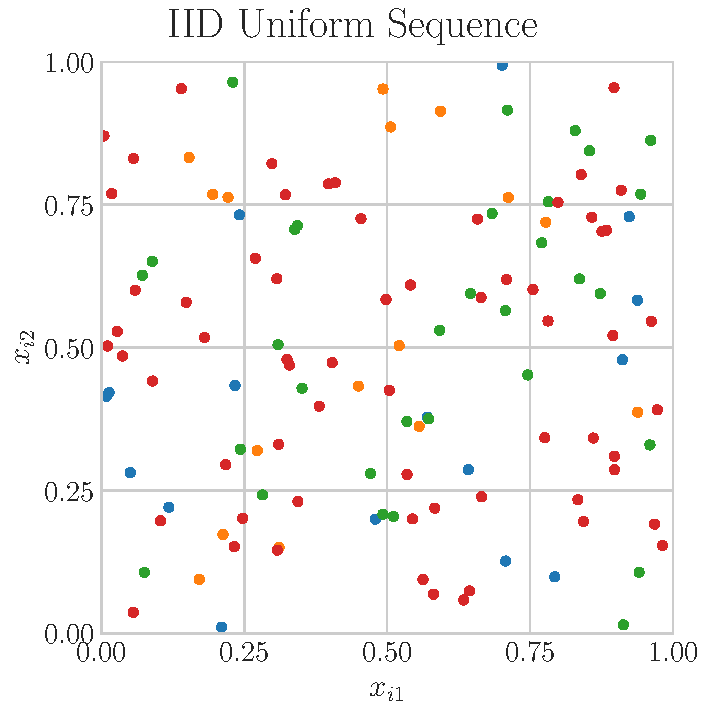
\includegraphics[width = 0.27\textwidth]{Figures/Uniform.pdf} \qquad 
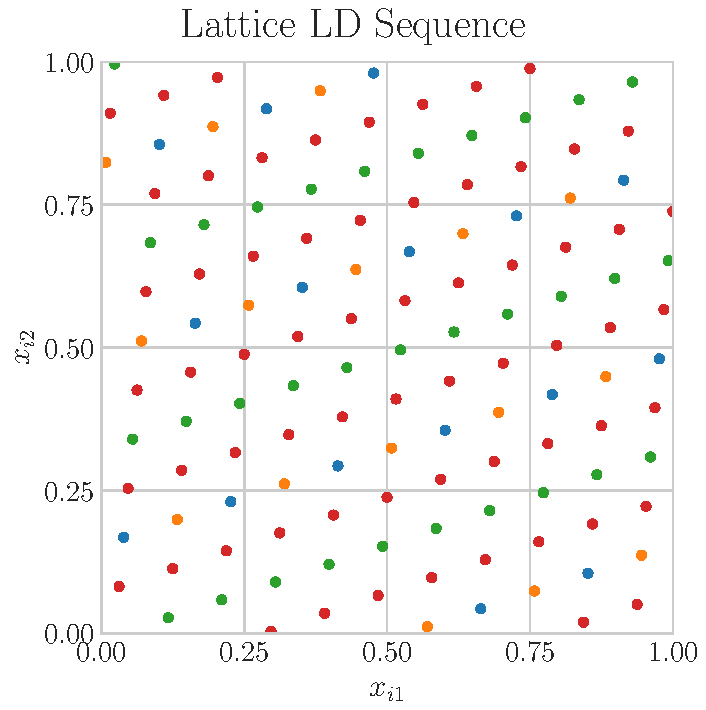
\includegraphics[width = 0.27\textwidth]{Figures/Lattice.pdf}
    \caption{Comparison of an IID sequence with a popular LD sequence.  Blue dots represent the first $16$ points, the orange dots the next $16$ points, the green dots the next $32$ points, and so on.  The lattice LD points are more evenly distributed than the IID points, which have clusters and gaps. \label{fig:points}}
\end{figure}

Figure \ref{fig:points} shows how LD sequences fill space more evenly than IID sequences.  The \emph{discrepancy}, $D\bigl(\{x_i\}_{i=1}^n\bigr)$,  \cite{Hic97a,Hic99a} is a quantitative measure of how close the empirical distribution of $\{x_i\}_{i=1}^n$ is to the uniform distribution.  Moreover, the error of QMC, $\lvert \mu - \hmu_n\rvert$, is bounded above by $D\bigl(\{x_i\}_{i=1}^n\bigr) \, \lVert f\rVert$, where  $\lVert f\rVert$ is a semi-norm of $f$, often called the \emph{variation}.  Different choices of the seminorm imply different definitions of the discrepancy.  LD sequences have small discrepancy.

The UNSW group has pioneered many innovations in the theory and application of QMC.

\section{Rigorous Adaptive Algorithms}
Although the discrepancy of a point set, $D\bigl(\{x_i\}_{i=1}^n\bigr)$ may often be computed, computing $\lVert f\rVert$ is harder than the original problem of computing $\mu=\int_{[0,1]^d} f(\vx) \, \dif \vx$.  Thus the error bound above is not suitable as a stopping criterion for determining the $n$ required to ensure that $\abs{\mu - \hat{\mu}_n}$ does not exceed a given error tolerance, $\varepsilon$.  Sometimes practitioners will use random replications of the point set, $\{x_i\}_{i=1}^n$, and use the standard deviation of the resulting random sample of $\hat{\mu}_n$ to estimate the error.

Hickernell and collaborators track the discrete Fourier (complex exponential) coefficients of the function data, $\{f(\vx_i)\}_{i=1}^n$ for lattice LD sequences $\{x_i\}_{i=1}^n$.  Under certain assumptions on the general decay of the true Fourier coefficients of $f$, one can construct theoretically justified stopping criteria for choosing $n$ to guarantee that $\abs{\mu - \hat{\mu}_n} \le \varepsilon$ \cite{JimHic16a}.  An analogous theory holds for digital sequences \cite{HicJim16a}.

Alternatively, one can assume that $f$ is an instance of a Gaussian process and construct credible intervals for $\mu$, which can be used to determine the sample size, $n$, required to meet the desired error tolerance.  In general, this approach requires expensive $\Order(n^3)$ matrix operations, but when suitable covariance kernels for the Gaussian process are matched with the LD lattice or digital net sequence, the computational burden reduces  to a very feasible $\Order(n \log(n))$ \cite{RatHic19a,JagHic22a}.

Hickernell and collaborators have also developed rigorous adaptive algorithms for IID Monte Carlo computation of $\mu$ \cite{HicEtal14a} and for univariate integration, approximation, and optimization \cite{ChoEtal17a,HicETal14b}.
%Software libraries in Matlab and Python that implement many of these adaptive algorithms have been developed by Hickernell and collaborators \cite{ChoEtal21a,QMCPy2020a}.  
The core assumption in all of these rigorous adaptive algorithms, is that $f$ belongs to a \emph{cone} of functions that are not too peaky.

\section{Proposed Activities During the Visit}

During the proposed visit to Sydney, Hickernell will give a series of several lectures on adaptive algorithms and QMC and the role of cones in constructing adaptive algorithms.  The focus will be to summarize what is known and identify several accessible research problems.  This includes the following:
\begin{itemize}
    \item The adaptive algorithms for QMC apply to a fixed dimension, $d$. Many interesting applications involve very large or even infinite $d$, which benefit from multilevel methods \cite{Gil14a}.  We will attempt to develop rigorous stopping criteria for multilevel methods, especially those that arise in the uncertainty quantification problems that Frances Kuo and her collaborators are experts in.

    \item The adaptive univariate integration algorithm seems ripe to be expanded to finite element methods with their a posteriori error bounds in one or more dimensions.  Many interesting applications involve partial differential equations with random coefficients.  We will explore these possibilities for constructing rigorous, adaptive algorithms.

    \item The lectures given by Hickernell may expose algorithms that the audience is developing that are amenable to the approach that Hickernell has used for developing adaptive stopping rules.  We will explore these possibilities.
\end{itemize}
The visit to University of Sydney will be July 20 -- August 2, 2026, with Professor Georg Gottwald as host.  The visit to University of New South Wales will be August 3--16, 2026, with Professor Frances Kuo as host.  %Follow up research after the visit will be carried out remotely or when we meet at professional conferences.

\bibliographystyle{amsplain}
\bibliography{FJH25,FJHown23}

\end{document}